%%%%%%%%%%%%%%%%%%%%%%%%%%%%%%%%%%%%%%%%%%%%%%%%%%%
%% P3: Phenomenology of Particle Physics                         
%%
%% Author:  André Rubbia                   		 
%%
%% Figure 27.17 Precision measurement of the $Z^0$ boson width at LEP.
%%
%% This work is licensed under the Creative Commons Attribution 4.0 International License. 
%% To view a copy of this license, visit http://creativecommons.org/licenses/by/4.0/ or 
%% send a letter to Creative Commons, PO Box 1866, Mountain View, CA 94042, USA.
%%
%%%%%%%%%%%%%%%%%%%%%%%%%%%%%%%%%%%%%%%%%%%%%%%%%%%

\documentclass[a4paper,10pt]{article}

\usepackage[T1]{fontenc}
\usepackage[utf8]{inputenc}
\usepackage{lmodern}
\usepackage[labelfont=bf]{caption}
\usepackage{upgreek}

\usepackage{tikz}
\usepackage{pgfplots}
\pgfplotsset{compat=1.17}
\usepgfplotslibrary{ternary}
\usepgfplotslibrary{fillbetween}
\usepgfplotslibrary{external}

\def\d{\mathrm{d}}
\setlength{\oddsidemargin}{-1.0cm}
\setlength{\evensidemargin}{-1.0cm}
\setlength{\textheight}{25cm}
\setlength{\textwidth}{18cm}

\pgfkeys{/pgf/number format/.cd,1000 sep={}}

\begin{document}

%%%%%%%%%%%%%%%%   FIGURE  %%%%%%%%%%%%%%%%%%%%%%%%%%%%%%
\begin{figure}[htb]
 	\centering
		\begin{tikzpicture}[scale=1]
%
% Z0 width
%
\begin{axis}[
    xbar,
    width=10cm,
    height=4cm,
    title={Total $Z^0$ width},
    xlabel={$\Gamma_Z$ (MeV)},
    symbolic y coords={ybot,average,OPAL,L3,DELPHI,ALEPH,ytop},
    ytick=data,
    ymin=ybot,ymax=ytop,
    xmin=2480, xmax=2530,
    legend pos=north east,
]
\addplot[
    color=blue,only marks,
    mark=*,
        error bars/.cd,
    x dir=both, x explicit
    ]
    coordinates {
    (2495.1,ALEPH)+-(4.3,0)
    (2487.6,DELPHI)+-(4.1,0)
    (2502.4,L3)+-(4.2,0)
    (2494.8,OPAL)+-(4.1,0)
    (2495.2,average)+-(2.3,0)
};
    \draw[gray,fill,fill opacity=0.2] (axis cs:2492.9,ybot) rectangle (axis cs:2497.5,ytop);
    \node at  (axis cs:2518,ALEPH) {$2495.1\pm4.3$~\cite{Barate:1999ce}};
    \node at  (axis cs:2518,DELPHI) {$2487.6\pm 4.1$~\cite{Abreu:2000mh}};
    \node at  (axis cs:2518,L3) {$2502.4\pm 4.2$~\cite{Acciarri:2000ai}};
    \node at  (axis cs:2518,OPAL) {$2494.8\pm 4.1$~\cite{Abbiendi:2000hu}};
    \node at  (axis cs:2518,average) {$2495.2\pm 2.3$};
\end{axis}
\end{tikzpicture}
	\caption{Precision measurement of the $Z^0$ boson width at LEP.
	The average value is from the PDG.}
\end{figure}
%
%%%%%%%%%%%%%%%%   END FIGURE  %%%%%%%%%%%%%%%%%%%%%%%%%%%%%%
%

\begin{thebibliography}{99}
\bibitem{Barate:1999ce}
R.~Barate {\em et~al.}, ``{Measurement of the Z resonance parameters at LEP},''
  {\em Eur. Phys. J. C}, vol.~14, pp.~1--50, 2000.

\bibitem{Abreu:2000mh}
P.~Abreu {\em et~al.}, ``{Cross-sections and leptonic forward backward
  asymmetries from the Z0 running of LEP},'' {\em Eur. Phys. J. C}, vol.~16,
  pp.~371--405, 2000.

\bibitem{Acciarri:2000ai}
M.~Acciarri {\em et~al.}, ``{Measurements of cross-sections and forward
  backward asymmetries at the $Z$ resonance and determination of electroweak
  parameters},'' {\em Eur. Phys. J. C}, vol.~16, pp.~1--40, 2000.

\bibitem{Abbiendi:2000hu}
G.~Abbiendi {\em et~al.}, ``{Precise determination of the Z resonance
  parameters at LEP: 'Zedometry'},'' {\em Eur. Phys. J. C}, vol.~19,
  pp.~587--651, 2001.
\end{thebibliography}

\end{document}
